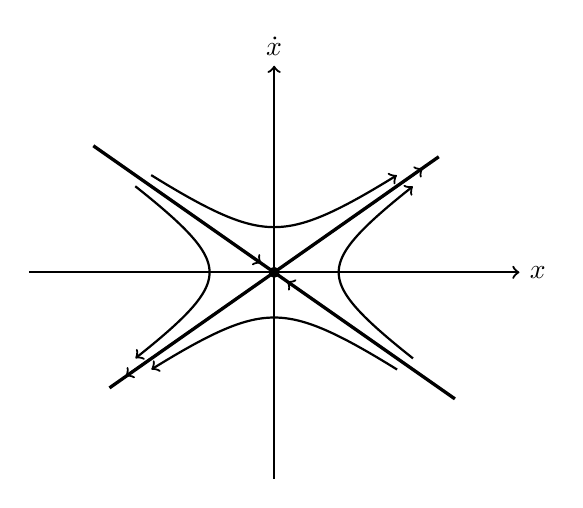
\begin{tikzpicture}[x=0.82cm,y=0.82cm,thick]
  \draw[->] (-3.8,0)--(3.8,0) node[right] {$x$};
  \draw[->] (0,-3.2)--(0,3.2) node[above] {$\dot x$};
  % Stable eigenline has negative slope; unstable eigenline has positive slope.
  \draw[very thick] (-2.8,1.96)--(2.8,-1.96);
  \draw[very thick] (-2.55,-1.79)--(2.55,1.79);
  \draw[->] (-2.5,1.75)--(-0.2,0.14); \draw[->] (2.5,-1.75)--(0.2,-0.14);
  \draw[->] (0.2,0.14)--(2.3,1.61); \draw[->] (-0.2,-0.14)--(-2.3,-1.61);
  % Hyperbolic sample orbits for one negative and one positive eigenvalue.
  \foreach \cOne/\cTwo in {0.5/0.5,0.5/-0.5,-0.5/0.5,-0.5/-0.5} {
    \draw[->] plot[domain=-2:2,samples=140,variable=\t]
      ({\cOne*exp(-0.7*\t)+\cTwo*exp(0.7*\t)},
       {-0.7*\cOne*exp(-0.7*\t)+0.7*\cTwo*exp(0.7*\t)});
  }
  \fill (0,0) circle (2pt);
\end{tikzpicture}
